\documentclass[11pt]{article}

\usepackage[a4paper,margin=2.35cm]{geometry}
\usepackage{fontspec}
\IfFontExistsTF{Times New Roman}
  {\setmainfont{Times New Roman}}
  {\setmainfont{Liberation Serif}}
\usepackage{amsmath}
\usepackage{booktabs}
\usepackage{caption}
\usepackage{float}
\usepackage{graphicx}
\usepackage{hyperref}
\usepackage{microtype}
\usepackage{tabularx}
\usepackage{xcolor}

\definecolor{linkblue}{HTML}{2F6F9F}
\definecolor{bodygray}{HTML}{333333}

\hypersetup{
  colorlinks=true,
  linkcolor=linkblue,
  citecolor=linkblue,
  urlcolor=linkblue
}

\captionsetup{font=small,labelfont=bf}
\setlength{\parindent}{0pt}
\setlength{\parskip}{0.62em}
\renewcommand{\arraystretch}{1.14}

\begin{document}

\setcounter{section}{1}
\section{Data Processing and Analysis}

\subsection{Purpose of This Chapter}

The previous part of the report identifies flight delay risk at John F. Kennedy International Airport (JFK) through the airport context, four core delay factors, and SWOT and PEST analysis. This chapter turns that qualitative risk language into a structured empirical dataset. It explains where the data come from, how the raw fields are cleaned, how frequency and severity variables are constructed, and what the main descriptive patterns imply for later operational risk modeling.

The chapter is therefore a bridge between risk identification and quantitative modeling. Weather, carrier operation, National Airspace System (NAS) pressure, and late-arriving aircraft are not treated only as narrative categories. They are translated into measurable event counts, delay-minute severity measures, and broader risk blocks that can support frequency models, severity models, dependence analysis, and aggregate operational risk simulation in the later sections of the project.

\subsection{Data Source and Sample Scope}

The project uses the U.S. Bureau of Transportation Statistics (BTS) On-Time Performance Airline Delay Cause dataset. The raw file contains monthly airline-level records, so each observation describes one airline's arrival operation at JFK in one calendar month. The working sample is restricted to JFK arrivals from January 2020 to December 2025. This multi-year window is useful because it includes both the pandemic disruption period and the later recovery years, giving the analysis enough variation to observe normal and stressed operating conditions.

The raw JFK extract contains 570 airline-month records. After the cleaning rules described below, 569 records remain. The final dataset covers 72 airport months and 12 airlines. Across the cleaned sample there are 657,671 arrival flights, 137,247 arrivals delayed by at least 15 minutes, 18,230 cancellations, 1,873 diversions, and 11,125,838 total arrival delay minutes. Table~\ref{tab:sample-coverage} summarizes the sample construction.

\begin{table}[H]
\centering
\caption{Sample coverage after data cleaning}
\label{tab:sample-coverage}
\begin{tabular}{lr}
\toprule
Metric & Value \\
\midrule
Raw JFK airline-month records & 570 \\
Cleaned airline-month records & 569 \\
Removed records with missing or zero arrival flights & 1 \\
Removed records with delayed arrivals exceeding total arrivals & 0 \\
Airport months covered & 72 \\
Airlines covered & 12 \\
Total arrival flights & 657,671 \\
Delayed arrivals, 15 minutes or more & 137,247 \\
Cancelled arrivals & 18,230 \\
Diverted arrivals & 1,873 \\
Total arrival delay minutes & 11,125,838 \\
\bottomrule
\end{tabular}
\end{table}

\subsection{Cleaning Logic and Output Datasets}

The cleaning procedure has four main steps. First, the raw BTS file and the official column-definition file are loaded and checked against the expected variables. Second, airline names are standardized so that the same airline is not split into multiple labels. For example, network-style names such as ``American Airlines Network'' and ``Delta Air Lines Network'' are converted into the more readable airline names used in the final tables. Third, technical BTS field names are rewritten into analysis-friendly names. For example, \texttt{arr\_flights} becomes \texttt{total\_arrival\_flights}, \texttt{arr\_del15} becomes \texttt{delayed\_arrivals\_15\_plus}, and \texttt{carrier\_delay} becomes \texttt{airline\_delay\_minutes}. Fourth, the workflow exports both full readable data and compact modeling inputs.

Two quality-control rules are especially important. Records with missing or zero total arrival flights are removed because they cannot produce meaningful delay rates, cancellation rates, or severity ratios. In the current sample, this removes one record, an Envoy Air observation in April 2020 with no usable operation volume. The workflow also checks whether delayed arrivals exceed total arrival flights. No such logical error is found, but the check is retained so that future dataset updates remain reproducible and defensible.

The processing pipeline generates several outputs. The readable full dataset preserves the main BTS fields with clearer labels. The core cleaned dataset keeps only the variables needed for modeling. The column dictionary links original BTS fields to readable names and plain-language definitions. The monthly summary supports trend analysis. The delay-cause summary supports risk-factor interpretation. The airline risk profile supports comparisons across airlines. Figure~\ref{fig:processing-panel} summarizes the pipeline and the main descriptive evidence in a report-ready format.

\begin{figure}[H]
\centering
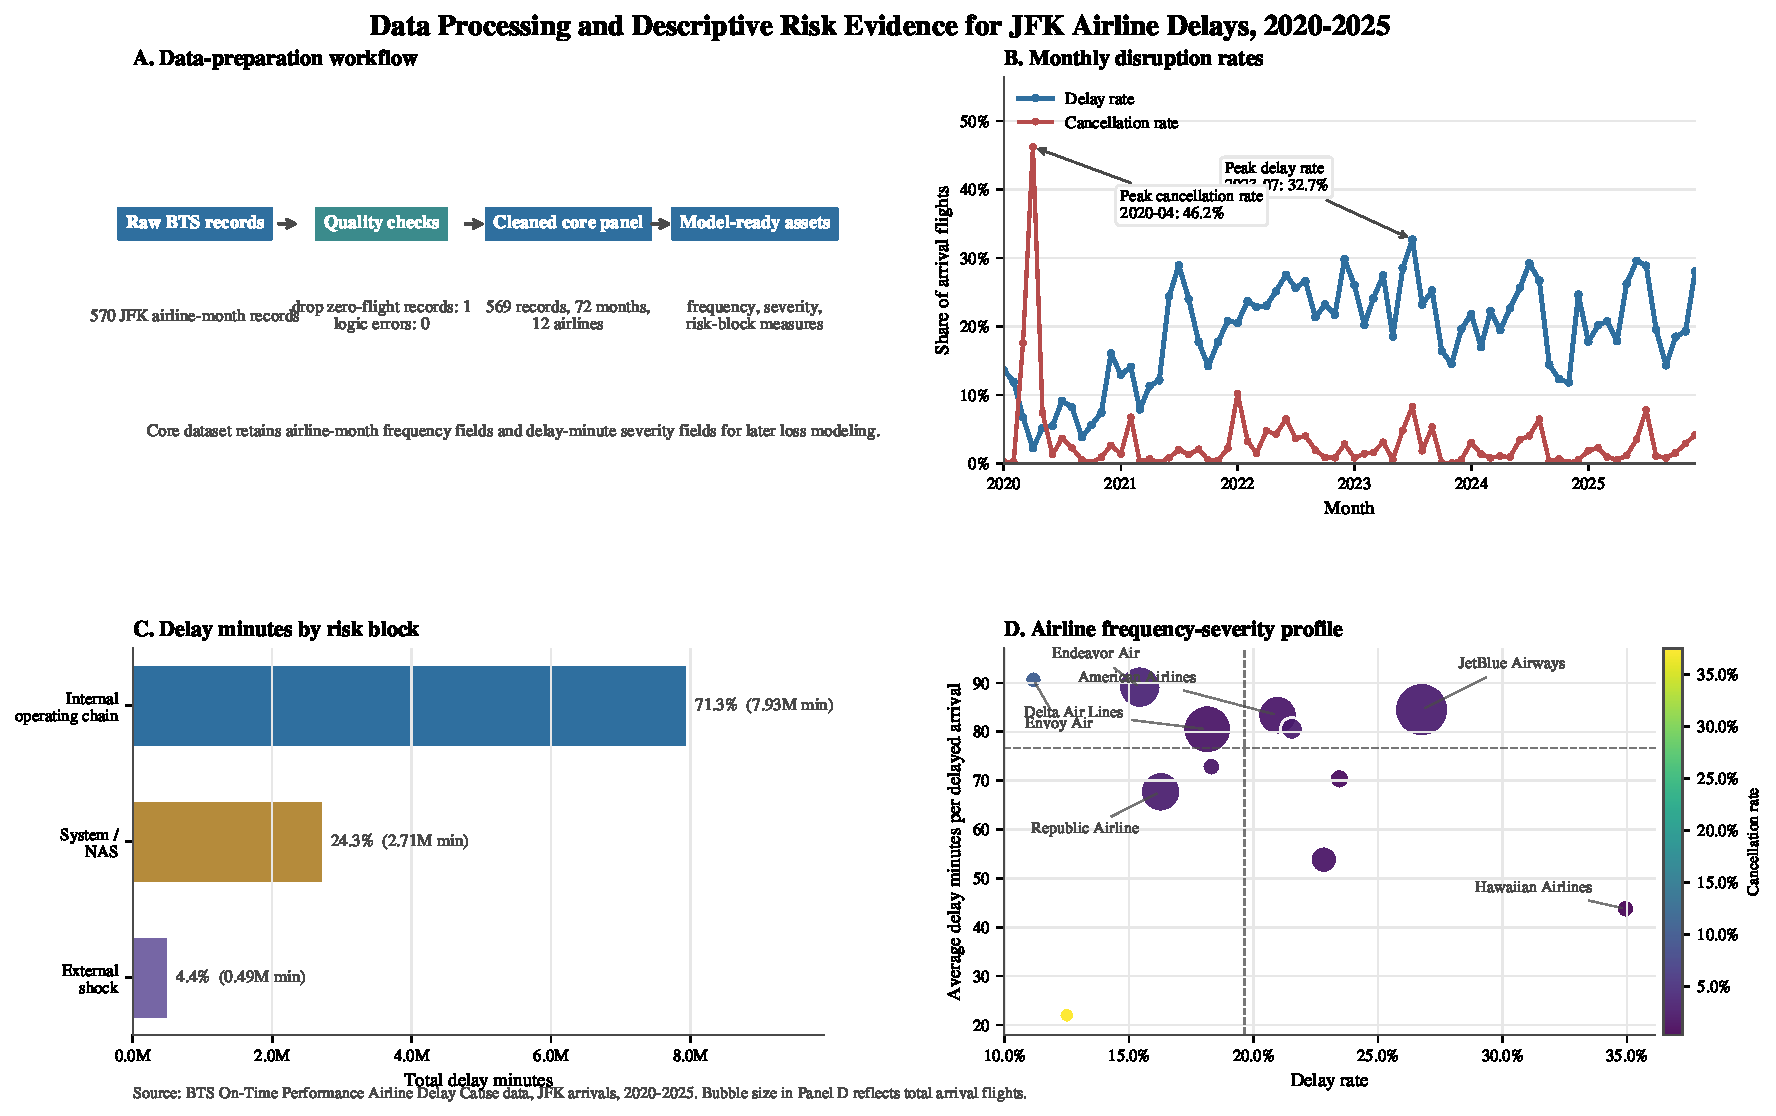
\includegraphics[width=\linewidth]{figures/jfk_data_processing_risk_panel.pdf}
\caption{Data processing and descriptive risk evidence for JFK airline delays, 2020--2025. Panel A summarizes the cleaning workflow. Panel B shows monthly delay and cancellation rates. Panel C aggregates BTS delay causes into the broader risk blocks used in the operational risk discussion. Panel D compares airlines by delay frequency, delay severity, cancellation rate, and operating volume.}
\label{fig:processing-panel}
\end{figure}

\subsection{Variable Design for Operational Risk Modeling}

The cleaned core dataset is organized around the standard operational risk distinction between event frequency and event severity. Frequency variables include total arrival flights, delayed arrivals, cancellations, and diversions. Severity variables include total arrival delay minutes and cause-specific delay minutes for Airline, Weather, NAS, Security, and Late Aircraft. Identifiers such as year, month, and airline name are retained so that the dataset can be analyzed by time and by airline.

At the airline-month level, the basic frequency ratios are
\[
\mathrm{DelayRate}_{a,t} =
\frac{\mathrm{DelayedArrivals}_{a,t}}{\mathrm{TotalArrivals}_{a,t}},
\qquad
\mathrm{CancellationRate}_{a,t} =
\frac{\mathrm{CancelledArrivals}_{a,t}}{\mathrm{TotalArrivals}_{a,t}}.
\]
The main severity measure is average delay minutes per delayed arrival:
\[
\mathrm{AverageSeverity}_{a,t} =
\frac{\mathrm{TotalDelayMinutes}_{a,t}}{\mathrm{DelayedArrivals}_{a,t}}.
\]
This separation is useful because the later modeling stage asks two different questions: how often disruption events occur, and how costly they are once they occur. A month with many short delays has a different operational meaning from a month with fewer but much longer delays.

For the broader risk framework, the original BTS causes are also mapped into three course-level risk blocks. Airline delay and Late Aircraft delay are grouped as internal operating-chain risk because both are closely connected to airline scheduling, aircraft rotation, crew availability, maintenance, and recovery buffers. NAS delay is treated as system constraint risk because it reflects air traffic flow, airport capacity, and broader network congestion. Weather and Security are grouped as external shock risk because they are less directly controlled by airlines and airport managers, even though their operational consequences still require preparation.

\subsection{Unified Operational Impact Measure}

Because the BTS dataset records cancellations and diversions as counts rather than minutes, the project uses delay-equivalent minutes as a common operational impact measure. For airline \(a\) in month \(t\), total operational impact is defined as
\[
L_{a,t} =
\mathrm{TotalDelayMinutes}_{a,t}
+ 180 \times \mathrm{CancelledArrivals}_{a,t}
+ 240 \times \mathrm{DivertedArrivals}_{a,t}.
\]
The 180-minute cancellation penalty and the 240-minute diversion penalty should be read as modeling proxies rather than exact passenger waiting times. They provide a transparent way to combine delays, cancellations, and diversions without making subjective monetary assumptions.

The choice of 180 minutes for cancellations is linked to the U.S. Department of Transportation tarmac-delay framework, under which airlines generally must give passengers on domestic flights at U.S. airports an opportunity to deplane before the three-hour point \cite{dot2025tarmac}. In passenger-rights practice, long delays are also treated as economically meaningful disruptions. EU Regulation 261/2004 covers cancellation and long-delay passenger rights, and official EU passenger-rights guidance uses a three-hour arrival-delay threshold for compensation in many cases \cite{eu2004reg261,euyoureurope2026}. For a hub such as JFK, a three-hour penalty is therefore a reasonable lower-bound proxy for the operational impact of a cancellation.

The diversion penalty is set higher, at 240 minutes, because a diversion usually implies a more complex recovery process. The aircraft has already departed, landed at an unplanned airport, and may require ground handling, refueling, passenger reprocessing, crew-duty adjustment, and a continuation leg or alternative transport. The DOT tarmac-delay framework also uses a four-hour threshold for international flights at U.S. airports \cite{dot2025tarmac}. Empirical aviation research on diversions due to in-flight medical emergencies reports that diverted flights often continue to their destination but impose additional delay and operating costs; one study summarized in TRID reports average direct operating and passenger time costs around USD 38,000 for medical-diversion cases, with nonmedical diversions taking longer to recover \cite{lewis2021diversions}. The ordering \(240 > 180\) therefore reflects the operational logic that diversions are usually more disruptive than cancellations.

\subsection{Descriptive Findings}

The cleaned data show that JFK's delay risk is not evenly distributed across time. The highest monthly delay rate occurs in July 2023, when 32.69\% of arrivals were delayed by at least 15 minutes and the month generated 395,899 delay minutes. The highest cancellation volume occurs earlier, in March 2020, with 1,900 cancellations, while the highest cancellation rate appears in April 2020 because the denominator of total flights fell sharply during the pandemic shock. This distinction matters for operational risk interpretation. Delay risk during normal or high-demand periods often reflects congestion and operating pressure, while cancellation spikes can also reflect major planning shocks and sharp reductions in flight volume.

The cause structure is concentrated. Airline and Late Aircraft delays together account for 7,933,073 delay minutes, or 71.30\% of total delay minutes. NAS contributes 24.32\%, while Weather and Security together contribute 4.38\%. Table~\ref{tab:cause-shares} reports the detailed BTS cause shares. The result does not mean that weather is unimportant. Rather, it means that in this monthly airline-level sample the largest day-to-day risk mass comes from the internal operating chain and from system congestion. Weather remains important as a trigger and tail amplifier, but it is not the dominant source of total recorded delay minutes.

\begin{table}[H]
\centering
\caption{Delay-minute contribution by BTS cause}
\label{tab:cause-shares}
\begin{tabular}{lrr}
\toprule
Cause & Delay minutes & Share of total delay minutes \\
\midrule
Airline & 4,022,961 & 36.16\% \\
Late Aircraft & 3,910,112 & 35.14\% \\
NAS & 2,705,624 & 24.32\% \\
Weather & 466,088 & 4.19\% \\
Security & 21,053 & 0.19\% \\
\bottomrule
\end{tabular}
\end{table}

Airline-level results add another layer of interpretation. JetBlue Airways contributes the largest total delay minutes in the sample, with 4.80 million delay minutes and 56,767 delayed arrivals. Delta Air Lines and American Airlines also contribute large total delay volumes because of their operating scale. Hawaiian Airlines has the highest delay rate, but its total number of arrivals is small, so it should not be interpreted in the same way as a large hub carrier. Envoy Air has the highest average delay severity, but it also has a very small operating base in the cleaned sample. Table~\ref{tab:airline-profile} reports the leading airline profiles by total delay minutes.

\begin{table}[H]
\centering
\caption{Selected airline risk profiles, sorted by total delay minutes}
\label{tab:airline-profile}
\begin{tabular}{lrrrr}
\toprule
Airline & Arrival flights & Delay rate & Cancellation rate & Avg. delay minutes \\
\midrule
JetBlue Airways & 212,172 & 26.76\% & 2.97\% & 84.5 \\
Delta Air Lines & 153,673 & 18.14\% & 1.99\% & 80.5 \\
American Airlines & 76,512 & 20.97\% & 2.31\% & 83.4 \\
Endeavor Air & 96,017 & 15.43\% & 3.84\% & 89.1 \\
Republic Airline & 82,768 & 16.27\% & 3.12\% & 67.7 \\
Alaska Airlines & 19,500 & 22.83\% & 2.01\% & 53.8 \\
\bottomrule
\end{tabular}
\end{table}

These patterns support the argument developed in the earlier risk-identification section. JFK delay risk is shaped by external conditions, but the largest measurable delay-minute burden in the dataset is linked to the airline operating chain and airport-system constraints. This is why the later quantitative model should not treat all delay causes as independent isolated events. It should preserve cause information while also allowing for broader risk blocks and state-dependent disruption patterns.

\subsection{Modeling Handoff and Limitations}

The cleaned outputs support the following modeling tasks. The core dataset can be used to fit frequency distributions for delayed arrivals, cancellations, diversions, and risk-block event counts. The severity variables can be used to fit delay-minute distributions, including average delay minutes per delayed arrival or cause-specific delay minutes. The monthly summary preserves chronological order, which supports normal-versus-disrupted state classification and later Markov transition analysis. Finally, the delay-equivalent impact measure \(L_{a,t}\) provides a common unit for aggregate risk simulation.

There are also limitations. The dataset is monthly and airline-level, so it cannot identify individual flight connections, hourly congestion, aircraft tail rotations, or exact weather-event timing. BTS cause fields are attribution measures based on reporting rules, not perfectly independent physical causes. Some small airlines have very few JFK arrivals, so their rates can be volatile and should be interpreted carefully. These limitations do not prevent the dataset from supporting the course project's quantitative analysis, but they define the level of precision that the later models can reasonably claim.

Overall, the data-processing stage creates an interpretable and reproducible empirical foundation for the rest of the report. It links the managerial risk categories discussed earlier with measurable frequency, severity, and aggregate-impact variables, making the later loss-modeling work an extension of the operational risk framework rather than a separate statistical exercise.

\begin{thebibliography}{9}

\bibitem{dot2025tarmac}
U.S. Department of Transportation. (2025). \emph{Tarmac delays}. Office of Aviation Consumer Protection. Retrieved May 17, 2026, from \url{https://www.transportation.gov/individuals/aviation-consumer-protection/tarmac-delays}

\bibitem{eu2004reg261}
European Parliament and Council. (2004). \emph{Regulation (EC) No 261/2004 establishing common rules on compensation and assistance to passengers in the event of denied boarding and of cancellation or long delay of flights}. Official Journal of the European Union. \url{https://eur-lex.europa.eu/eli/reg/2004/261/oj}

\bibitem{euyoureurope2026}
European Union. (2026). \emph{Air passenger rights}. Your Europe. Retrieved May 17, 2026, from \url{https://europa.eu/youreurope/citizens/travel/passenger-rights/air/index_en.htm}

\bibitem{lewis2021diversions}
Lewis, B. A., Gawron, V. J., Esmaeilzadeh, E., Mayer, R. H., Moreno-Hines, F., Nerwich, N., \& Alves, P. M. (2021). Data-driven estimation of the impact of diversions due to in-flight medical emergencies on flight delay and aircraft operating costs. \emph{Aerospace Medicine and Human Performance, 92}(2), 99--105. \url{https://doi.org/10.3357/AMHP.5720.2021}

\end{thebibliography}

\end{document}
